\graphicspath{ {Figures/chapter03} }
\section{System Schematics}
The Ball and Plate (BPS) system is unstable, nonlinear, multi-variable, and under-actuated, The BPS model is an extension of the classical Ball and Beam system. It consists of a rectangular flat plate fixed movable at its center by a universal joint. The control target is the plate which could rotate about 2 mutually perpendicular axes
\begin{figure}[h]
\centering
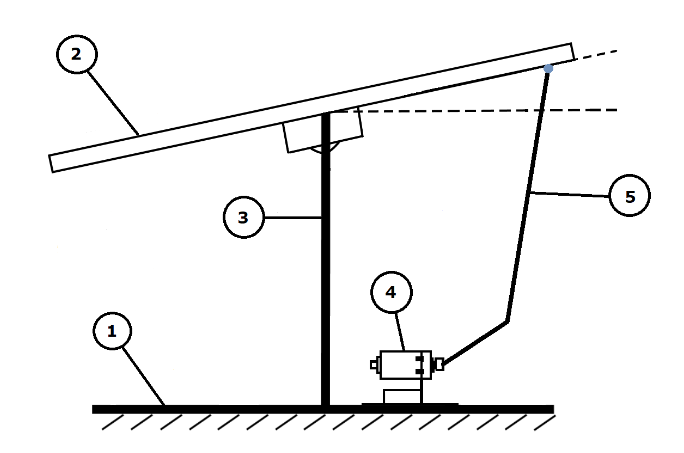
\includegraphics[width=0.5\textwidth]{BPS2DView}
\caption{Side projection of a BPS}
\end{figure}
The mechanical parts of the BPS are illustrated in Fig. 2.1, which contains;
\begin{enumerate}
\item The BPS wooden base carries all the other components of the system.
\item Plate is a plastic holder and a resistive touch screen sensor.
\item The central shaft is used between the structure base and the middle of the plate holder. Its job is to hold the plate from the center point by a connected universal joint.
\item The servo motor holder which fits the main base.
\item Two independent two-linkage mechanism which is used to convert rotation motion from servo motor to linear motion in the plate
\end{enumerate}


\section{Plant modeling}
The mathematical model of any mechanical system can be derived using three
Methods;
\begin{enumerate}
 \item The classical Newton method 
 \item Modern Euler-Lagrange method
 \item Hamiltonian mechanics method
 \end{enumerate}
In our study, we will use the second method to derive the system's equations of motion and we will compare them with simcape to verify their validity
\subsection{Requirements and assumptions}
Before deriving the mathematical model of BPS, it's essential to begin by setting a standing point to take into account during the mathematical analysis. First, the model as shown in Fig. 2.2 will be divided into two models, a ball and plate model and a servo motor model therefore the following assumptions are made
\begin{enumerate}
    \item The ball and the plate are in continuous contact.
    \item All friction forces and rotational moments are neglected.
    \item The ball is completely symmetric and rounded.
    \item The ball is not sliding.
\end{enumerate}
\begin{figure}[h]
\centering
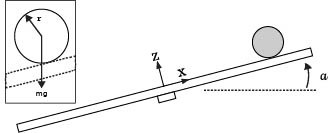
\includegraphics[width=0.7\textwidth]{sss.jpg}
\caption{Schematic representation of the Ball and Plate System (BPS).}
\end{figure}
\subsection{Euler-Lagrange approach}
In this section, the mathematical model of BPS is developed based on the Euler–Lagrange equation \cite{nokhbeh2011modelling}.
The relation between the kinetic and the potential energy
possessed by the mechanical system is described by the following
equation.

\begin{equation}
L(q_i, \dot{q_i}, t) = T( \dot{q_i}, t) - V( q_i, t) 
\end{equation}
where $L $ is the Lagrangian function which represents the
difference between the overall kinetic energy $T$ and the overall potential
energy $V$. Then, the general Euler–Lagrange’s equation is
defined as:
\begin{equation}
\dv{t} \pdv{T}{\dot{q_i}} - \pdv{T}{q_i} + \pdv{V}{q_i} = Q_i    
\end{equation}
Equation (3.2) can express the motion of a wide variety of
mechanical systems where Qi represents the i-th generalized composite force acting on the system and qi is i-th generalized coordinate.\\

The system has 4 degrees of freedom therefore four generalized coordinates; two in ball motion \([x,y]\) and two in the inclination of the plate\([\alpha, \beta]\). Here we assume the generalized coordinates of the system to be $x$ and $y$ ball’s position on the plate and $\alpha$ and $\beta$ the inclination of the plate 
\[ q_i \in \{ x,y,\alpha,\beta\}  \]
The kinetic energy of the system consists of the kinetic energy of the ball and the kinetic energy of the plate
\begin{equation} T  = T_b + T_p  \end{equation}
While the kinetic energy of the ball consists of rotational with respect
to its center of mass and translational parts:
\begin{equation}T_b  = T_{trans} + T_{rot}  \end{equation}
 The translational energy of the ball can be described by: 
\begin{equation} T_{trans} = \frac{1}{2}m_b(v^2) = \frac{1}{2}m_b(\dot{x}^2 +\dot{y}^2)   \end{equation}
 The rotational energy of the ball :
\begin{equation}T_{rot} = \frac{1}{2}J_b\omega^2 = \frac{1}{2}J_b\frac{v^2}{r^2} = \frac{1}{2}\frac{J_b}{r^2}(\dot{x}^2 +\dot{y}^2)  \end{equation}
 

Where $m_b$ is mass of the ball and $J_b$ is moment of inertia of the ball; $\dot x$ and $\dot y$ are ball’s translational velocities along x-axis and y-axis; $\omega_x$ and $\omega_y$ are ball’s
rotational velocities along x-axis and y-axis that 
\begin{equation}
\omega_y = \frac{\dot{y}}{r_b} \quad  , \quad  \omega_x = \frac{\dot{x}}{r_b}  
\end{equation}
By substituting  (3.6) and (3.5) into equations
(3.4) we will have:
\begin{equation}
T_b = \frac{1}{2}m_b(\dot{x}^2 +\dot{y}^2) +
\frac{1}{2}\frac{J_b}{r^2}(\dot{x}^2 +\dot{y}^2) =
\frac{1}{2} \left( m_b + \frac{J_b}{r_{b}^2} \right) (\dot{x}^2 +\dot{y}^2)   
\end{equation}

the kinetic energy of the plate, by considering the ball as a point mass which is placed in ($x, y$) can be expressed as: 
\begin{equation}
T_p = \frac{1}{2} (J_b + J_p) \left( \dot{\alpha}^2 +\dot{\beta}^2 \right) + \frac{1}{2} m_b \left( x\dot{\alpha} + y\dot{\beta} \right)^2 
\end{equation}
From $T_b$ (3.8) and $T_p$ (3.9)  we can calculate the total kinetic energy by substituting into Eqs (3.3):

  \begin{equation}
          T= \frac{1}{2} \left( m_b + \frac{J_b}{r_b^2} \right)(\dot{x}^2 + \dot{y}^2 ) + \frac{1}{2} (J_p + J_b) \left(\dot{\alpha}^2 + \dot{\beta}^2 \right) + \frac{1}{2}m_b \left(  x\dot{\alpha} + y\dot{\beta} \right)^2
  \end{equation} 
  \\
 The potential energy $V$ of the ball according to the plate center can be calculated as:
\begin{equation}
V_b = m_bgh = m_bg(x\sin{\alpha} + y\sin{\beta})  
\end{equation}
Now the Lagrangian function can be expressed using equation (3.1):

    \begin{multline}
    L = \frac{1}{2} \left( m_b + \frac{J_b}{r_b^2} \right)(\dot{x}^2 + \dot{y}^2 ) + \frac{1}{2} (J_p + J_b) \left(\dot{\alpha}^2 + \dot{\beta}^2 \right) \\ + \frac{1}{2}m_b \left(  x\dot{\alpha} + y\dot{\beta} \right)^2  -m_bg(x\sin{\alpha} + y\sin{\beta})  
    \label{aaa}
    \end{multline}

Then we derive the system's equations 

\begin{align}\label{eq:lnnonspbb}
\pdv{T}{\dot{\alpha}} = (J_p + J_b) \dot{\alpha} + m_b \left(x^2\dot{\alpha} + yx\dot{\beta}\right) \\             
\pdv{T}{\dot{\beta}} = (J_p + J_b) \dot{\beta} + m_b \left(xy \dot{\alpha} + y^2\dot{\beta}\right) 
\end{align}


\begin{align}\label{eq:lnnonspbb}
 \pdv{T}{\dot{x}} = \left(m_b + \frac{J_b}{r^2}\right)\dot{x} \\
 \pdv{T}{\dot{y}} = \left(m_b + \frac{J_b}{r^2}\right)\dot{y} 
\end{align}
\begin{align}
\pdv{T}{x} = m_b \left( x\dot{\alpha} + y\dot{\beta} \right)\dot{\alpha} , \qquad 
\pdv{T}{y} = m_b \left( x\dot{\alpha} + y\dot{\beta} \right)\dot{\beta} 
\end{align}
\begin{align}\label{eq:aa3}
 \pdv{T}{\alpha} = 0 ,\quad 
  \pdv{T}{\beta} = 0
\end{align}

\begin{align}\label{eq:lnnonspbb}
 \pdv{V}{\alpha} = m_bgx\cos{\alpha} ,\quad 
 \pdv{V}{\beta} = m_bgy\cos{\beta} ,\quad 
\pdv{V}{x} = m_bgx\sin{\alpha} ,\quad 
 \pdv{V}{y} = m_bgy\sin{\beta} 
\end{align}

From the Lagrange-Euler equation of the ball, we can write:
\begin{equation}
    \dv{}{dt} \pdv{T}{\dot{x}} - \pdv{L}{x} =(m_{b}+\frac{J_{b}}{r_{b}^{2}})\ddot{x}-m_{b}(x\dot{\alpha}+y\dot{\beta})\dot{\alpha}+m_{b}g\sin\alpha=0
\end{equation} 
\begin{equation}
\dv{}{dt} \pdv{T}{\dot{y}} - \pdv{L}{y} =(m_{b}+\frac{J_{b}}{r_{b}^{2}})\ddot{y}-m_{b}(x\dot{\alpha}+y\dot{\beta})\dot{\alpha}+m_{b}g\sin\beta=0
\end{equation}
It is important to note there are no external forces (except gravity) acting on the ball itself
$(Q_x = 0$ and $Q_y = 0)$ and there are forces in the form of torque acting on the plate and changing its inclination $(Q_{beta} = \tau_y $ and $ Q_{alpha} =\tau_x )$. 
\begin{align} \label{eq:asdf}
\dv{}{dt} \pdv{T}{\dot{\alpha}} - \pdv{L}{\alpha} = 
(J_b + J_p)\ddot{\alpha} + m_bx^2\ddot{\alpha} + 2m_bx\dot{x}\dot{\alpha}\\ \nonumber
+m_bxy\ddot{\alpha} +m_b\dot{x}y\dot{\beta} + m_bx\dot{y}\dot{\beta} - m_bg\cos{\alpha}
=\tau_x   
\end{align}

\begin{align} \label{eq:asdf}
\dv{}{dt} \pdv{T}{\dot{\beta}} - \pdv{L}{\beta} = 
(J_b + J_p)\ddot{\beta} + m_by^2\ddot{\beta} + 2m_by\dot{y}\dot{\beta}\\ \nonumber
+m_bxy\ddot{\beta} +m_b\dot{y}x\dot{\alpha} + m_by\dot{x}\dot{\alpha} - m_bg\cos{\beta}
=\tau_x  
\end{align}
So the 4 differential equations of the BPS are respectively (3.20),(3.21),(3.22),(3.23), finally we rewrite these non-linear equations so we got:
\begin{equation}
    0 =\left( m_b + \frac{J_b}{r^2} \right)\ddot{x} - m_b \left( x\dot{\alpha}^2 + y\dot{\alpha}\dot{\beta}\right) + m_bg\sin{\alpha}
\end{equation}
\begin{equation}
    0 = \left( m_b + \frac{J_b}{r^2} \right)\ddot{y} - m_b \left(  x\dot{\beta}^2 + x\dot{\alpha}\dot{\beta}\right) + m_bg\sin{\beta} 
\end{equation}
\begin{align}\label{eq:asdf}
\tau_x &= 
(J_b + J_p + m_bx^2)\ddot{\alpha}  + 2m_bx\dot{x}\dot{\alpha} +m_bxy\ddot{\beta}\\ \nonumber
&+m_b\dot{x}y\dot{\beta} + m_bx\dot{y}\dot{\beta} - m_bgx\cos{\alpha}
\end{align}
\begin{align}\label{eq:asdf}
\tau_y &= 
(J_b + J_p + m_by^2)\ddot{\beta}  + 2m_by\dot{y}\dot{\beta} +m_bxy\ddot{\alpha}\\ \nonumber
&+m_b\dot{x}y\dot{\alpha} + m_bx\dot{y}\dot{\alpha} - m_bgy\cos{\beta}
\end{align}
It can be seen that equations (3.24) and (3.25) describe the ball motion and how the acceleration of the ball depends on its position on the plate and on angles and angular velocities of the plate. Equations (3.26) and (3.27) show plate dynamics and how it depends on external torques, ball position, velocity, angular velocity and acceleration of the plate.

It is necessary to note that dynamics of the stepper motors are neglected, thus the system equations describe only the ball and plate problem. These dynamics will be added in the geometrical analysis subsection later, however  we should know that it's assumed stepper motors don’t lose any step and load doesn’t
affect their performance thus equations (3.26) and (3.27) can be neglected

Then we can transform the model into state space form, defining state variables $X=(x_1,x_2,x_3,x_4,x_5,x_6,x_7,x_8) = (x,\dot{x},\alpha,\dot{\alpha},y,\dot{y},\beta,\dot{\beta})$
and from eqs (3.24), (3.25) we can get the nonlinear BPS's state equations as follows:\\ 
\begin{equation}
\begin{bmatrix}
\dot{x_1}\\
\dot{x_2}\\
\dot{x_3}\\
\dot{x_4}\\
\dot{x_5}\\
\dot{x_6}\\
\dot{x_7}\\
\dot{x_8}\\
\end{bmatrix}
=
\begin{bmatrix}
x_2\\
\frac{m_b}{m_b+\frac{j_b}{r^2}}(x_1x_4^2+x_4x_5x_8-g\sin{x_3})\\
x_4\\
0\\
x_6\\
\frac{m_b}{m_b+\frac{j_b}{r^2}}(x_5x_8^2+x_1x_4x_8-g\sin{x_7})\\
x_8\\
0\\
\end{bmatrix}
+ 
\begin{bmatrix}
0 & 0 \\
0 & 0 \\
0 & 0 \\
1 & 0 \\
0 & 0 \\
0 & 0 \\
0 & 0 \\
0 & 1 \\
\end{bmatrix}
\begin{bmatrix}
u_x  \\
u_y  \\
\end{bmatrix}
\end{equation}



\subsection{Interpretation of terms in system equations}
In the Table no. 3.1 description of the terms in the system equation and there units
\begin{table}[h]
  \centering
  \caption{Interpretation of mathematical model terms}
  \begin{tabular}{ | m{8em} | m{20em}| m{1cm} | } 
  \hline
  parameter & description & unit \\ 
  \hline  \hline
   $m_b$& Mass of the ball & kg \\ 
  \hline
  $r_b$ & Radius of the ball & m \\ 
  \hline
  $J_b$ & Moment of inertia of the ball & kgm2 \\   
  \hline
  $J_p$ & Moment of inertia of the plate & kgm2 \\   
  \hline
  $x,y$ & Coordinates of the ball from the center of the plate & m \\ 
  \hline
  $\dot{x},\dot{y}$ & First time derivatives of coordinates which represents the transitional velocity  & ms-1\\   
  \hline
  $\ddot{x},\ddot{y}$ & Second time derivatives of coordinates which represents the transitional acceleration & ms-2\\   
  \hline
  $\alpha , \beta$ & Plate inclination angles & rad \\   
  \hline 
  $\dot{\alpha},\dot{\beta}$ & First-time derivatives of plate angles which represents the angular velocity & rads-1 \\   
  \hline  
  $\ddot{\alpha},\ddot{\beta}$ & Second-time derivatives of plate angles which represent the angular acceleration & rads-2 \\   
  \hline  
  $\tau$ & Torques acting on the plate & Nm \\   
  \hline
  $g$ & Gravitational acceleration  & M/s2 \\  
  \hline
  $ m_b ( x\dot{\alpha}^2+y\dot{\alpha}\dot{\beta})$ & Centrifugal force  & N \\  
  \hline
  $(J_b+J_p+m_bx^2)\ddot{\alpha} $ & Gravitational acceleration  & Nm \\  
  \hline
  $ 2m_bx\dot{x}\dot{\alpha}$ & Coriolis influence   & Nm \\  
  \hline
  $m_bgx\cos{\alpha}$ & Gravitational influence  & Nm \\  
  \hline
  \end{tabular}

\end{table}

\section{Linearization and simplfication}

To simplify and linearize the model, four main assumptions was made 
\begin{enumerate}
    \item the stepper motors don’t lose any step and load doesn’t affect their performance.
    \item The ball is assumed to be a homogenous and solid sphere
    \item The rate of change of angles is close to zero.
    \item The angles of the plate are assumed to change in range 〈-15; 15〉 or in other words, $|\alpha| < 1$ and $|\beta| < 1$ in radians.
\end{enumerate}
In the interest of model simplification, the first assumption is made that stepper motors exhibit no step loss, and the impact of the load on their performance is discounted. Consequently, angles $|\alpha|$ and $|\beta|$ are deemed direct inputs to the system. Accordingly, equations (3.26) and (3.27) may be excluded and neglected from consideration as we said before.

Secondly to find the $\frac{m_b}{m_b+\frac{j_b}{r^2}}$ term we assumed the ball to be a  solid sphere, to find  $(J_b)$ of this sphere the approximate expression for a moment of inertia of a solid ball $(J_b)$ can be derived by summing the moments of fragile disks about z-axis as can be seen in fig. 3
\begin{figure}[h]
\centering
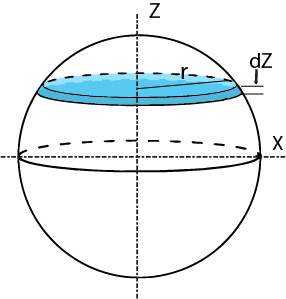
\includegraphics[width=0.4\textwidth]{SolidBallSegments.jpg}
\caption{Illustration of the moment of inertia calculation for solid ball segments}
\end{figure}
The moment of inertia expression for one disk $dJ$ derived by:
\begin{equation}
dJ = \frac{1}{2} r^2 dm = \frac{1}{2}r^2pdV = \frac{1}{2}r^2p\pi r^2dz 
\end{equation}
the mass of the disk $dm$ can be represented as the density of the ball $p$ times the volume of the disk $dV$, the volume can be represented as the disk area multiplied by the height $dz$.
To find the sum of the moment of inertia for all disks we integrate both sides of the equation to become:
\begin{equation}
J = \frac{1}{2}p\pi \int_{-R}^{R} r^4 \,dz \ = \frac{1}{2}p\pi \int_{-R}^{R} (R^2-z^2)^2 \,dz \ = \frac{8}{15} p\pi R^5 \end{equation}

 Where R is the Radius of the sphere and $y = (R^2-z^2)$ is derived from the Pythagorean theorem.
 Substituting the density expression $p = \frac{M}{V} = \frac{M}{\frac{4}{3}\pi R^3}$ gives:
\begin{equation}
J = \frac{8}{15}\left[  \frac{M}{\frac{4}{3}\pi R^3} \right]\pi R^5 
\end{equation}

 \begin{equation}
J = \frac{2}{5}MR^2 
\end{equation}
 So, as has been proven the approximate moment of inertia value for a solid ball is $J_b = \frac{2}{5}MR^2$, therefore by taking the account of all simplfications and substituting (3.32) into the system model we get:
\begin{equation}
\begin{bmatrix}
\dot{x_1}\\
\dot{x_2}\\
\end{bmatrix}
=
\begin{bmatrix}
x_2\\
\frac{5}{7}(-g\sin{x_3})\\
\end{bmatrix}
+ 
\begin{bmatrix}
0 \\
1 \\
\end{bmatrix}
\begin{bmatrix}
u_x  \\
\end{bmatrix}
\end{equation}

\begin{equation}
\begin{bmatrix}
\dot{x_5}\\
\dot{x_6}\\
\end{bmatrix}
=
\begin{bmatrix}
x_6\\
\frac{5}{7}(-g\sin{x_7})\\
\end{bmatrix}
+ 
\begin{bmatrix}
0  \\
1  \\
\end{bmatrix}
\begin{bmatrix}
u_y  \\
\end{bmatrix}
\end{equation}

It is assumed that the ball is rolling without slipping in continuous contact with the plate keeping in mind the rate of change of angles is low and close to zero, and because of that the angular velocity and the acceleration of the the plate rotation will be very low and can be negligible,
\[ \dot{\alpha} \approx 0 \]\[ \dot{\beta} \approx 0  \]

the last assumption to finally linearize the model is that the angle of inclination for the plate is relatively small (up to ± 15) which leads $\longrightarrow  \sin{\alpha} \simeq \alpha, \, \sin{\beta} \simeq \beta$ in rads so the final linearized equation will be
\begin{equation}    
\begin{bmatrix}
\dot{x_1}\\
\dot{x_2}\\
\end{bmatrix}
=
\begin{bmatrix}
x_2\\
0\\
\end{bmatrix}
+ 
\begin{bmatrix}
0 \\
\frac{5}{7}(-g) \\
\end{bmatrix}
\begin{bmatrix}
\alpha \\
\end{bmatrix}
\end{equation}

\begin{equation}
\begin{bmatrix}
\dot{x_5}\\
\dot{x_6}\\
\end{bmatrix}
=
\begin{bmatrix}
x_6\\
0\\
\end{bmatrix}
+ 
\begin{bmatrix}
0  \\
\frac{5}{7}(-g)  \\
\end{bmatrix}
\begin{bmatrix}
\beta  \\
\end{bmatrix}
\end{equation}

Equation No. (3.35) serves as the foundational equation for the subsequent steps in our process. Following these simplifications, the system equations can be expressed in transfer function form:
\begin{equation}\ddot{x} +\frac{5}{7}g \alpha = 0 \end{equation}
\begin{equation}\ddot{y} +\frac{5}{7}g \beta = 0 \end{equation}
Assuming the angles as inputs to BPS, the linearized transfer function can be obtained as:
\begin{equation}     G(s) = \frac{x(s)}{\alpha(s)} = -\frac{5}{7}\frac{g}{s^2} \end{equation}
\begin{equation} G(s) = \frac{y(s)}{\beta(s)} = -\frac{5}{7}\frac{g}{s^2} \end{equation}

To validate our linearization process, we compared the linear model with non-linear simulink and Simscape models through an open-loop step response by the Simulink program, using four different inputs, as presented in Figure 3.4. Since the system is open-loop, the response is unstable, and we can also notice from the figure that the difference between the three models increases as the angle of the plate \(\alpha\) increases. This is due to our assumption that the input angle changes in the range 〈15; 15〉.

\begin{figure}[h]
    \centering
    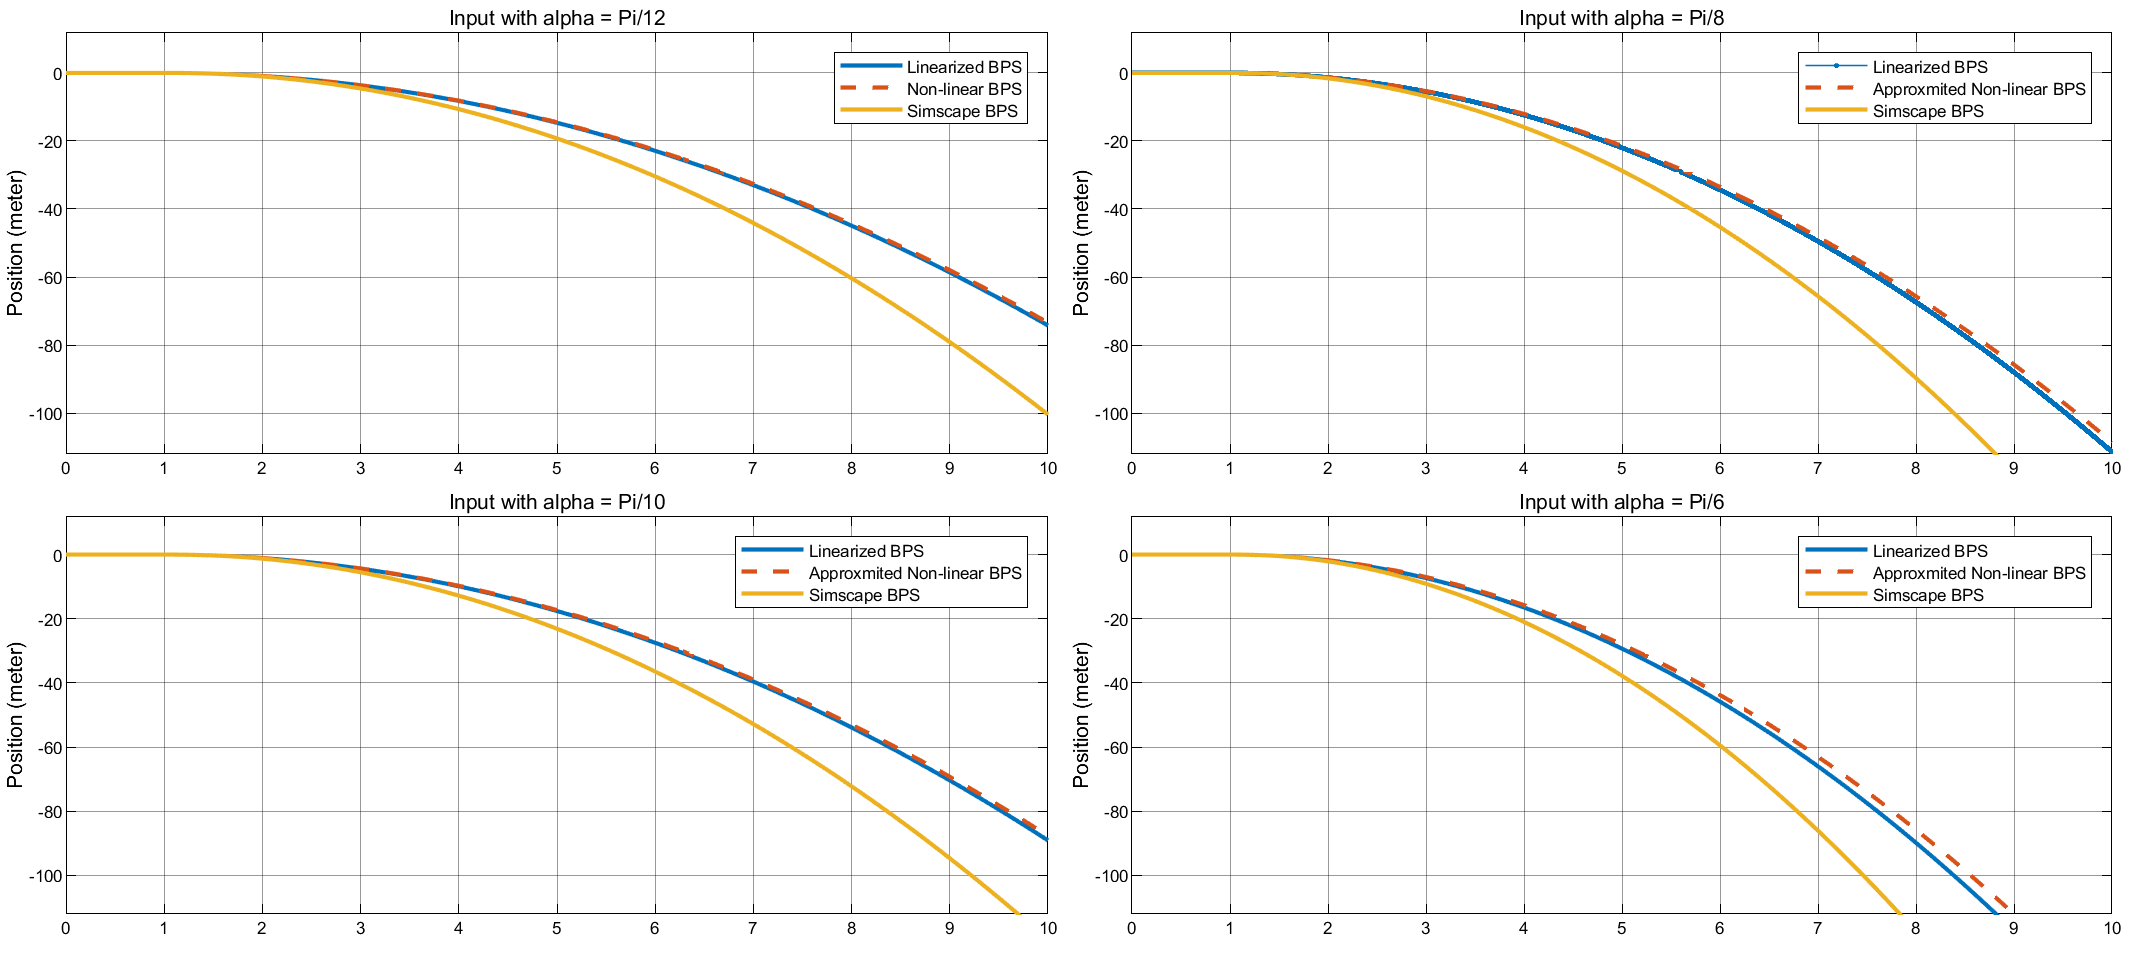
\includegraphics[width=1\textwidth]{Openl_loop_response_of_BPS_for_contant angle}
    \caption{Comparison of open-loop responses for linear, non-linear, and Simscape BPS models}
\end{figure}

\section{Geometrical analysis}
Since our overall system input should be the angle signal provided to the servo motor, not the plate inclination angle itself, we should discover the transfer function of the servo motor and then we should determine the gain or geometrical relationship between the plate inclination angle and servo motor angle
\subsection{Servo motor modeling}
Servomotors, like the MG995 model that we used in our thesis, are widely used for precise linear or angular motion in engineering. In Fig. 3.5, key components of the MG995 are highlighted. The DC motor generates rotational motion from applied voltage, while the gearbox adjusts speed and boosts torque. The electronic control board interprets PWM signals, converts them to angles, and computes control signals by comparing them with the current angle. Unlike professional servos with encoders, inexpensive hobby servos, including china made MG995's, often lack encoders and instead use a potentiometer for position sensing. The potentiometer, rotating with the output shaft, induces a voltage signal variation sent to the control board. This signal goes as a feedback and helps the internal controller calculate the difference between the desired and current positions, serving as the input for the embedded controller \cite{santanacob}.
\begin{figure}[h]
    \centering
    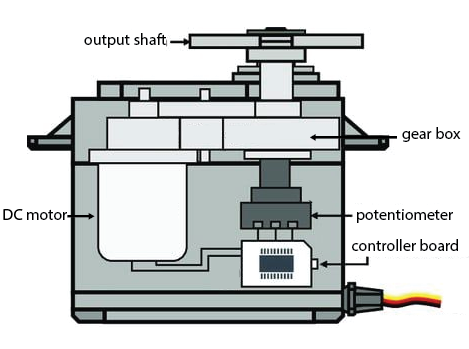
\includegraphics[width=0.5\textwidth]{servomotor_schematic.png}
    \caption{Schematic representation of key components in the MG995 servomotor}
\end{figure}
In the electrical dynamics of Fig. 3.6, key parameters include \(u\) (voltage applied), \(i\) (electrical current), \(R\) (motor resistance), \(L\) (inductance), and \(e\) (back electromotive force). On the mechanical side, \(\tau_m\) denotes motor torque, \(\tau_{jm}\) is motor moment of inertia, \(b_m\) is viscous friction coefficient, \(\tau_f\) is viscous friction torque, \(\theta_m\) is motor shaft rotation angle, N is gearbox gear ratio, \(J_l\) is load moment of inertia, \(\tau_l\) is load torque, and \(\theta_l\) is servo output shaft rotation angle.
\begin{figure}[h]
    \centering
    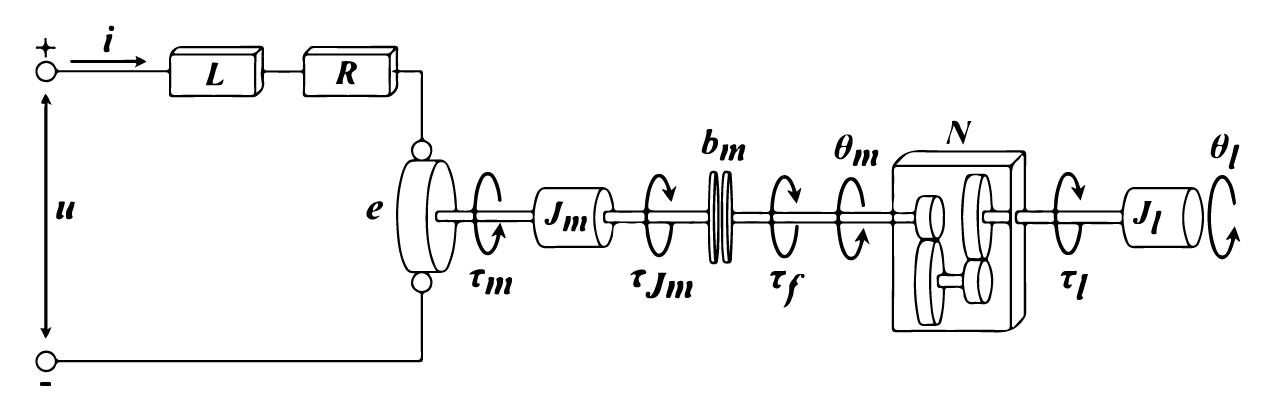
\includegraphics[width=0.8\textwidth]{Servomotor_dynamical_diagram}
    \caption{The electromechanical diagram of a servomotor system}
\end{figure}
 To obtain a transfer function that represents the open-loop dynamics $P(s)$ of a servo motor for a voltage input $U(s)$ and as output the angle of the servo output shaft $\Theta_l(s)$, is given by:

\begin{equation}P(s) = \frac{\Theta_l(s)}{U(s)} = \frac{K_t K_\omega \eta}{(J_{eq}s^2 + b_{eq}s)}
\end{equation}

 where $K_t$ is the motor torque constant, $K_\omega$ is the speed constant, and $\eta$ is the gearbox efficiency factor, $J_{eq} = J_l + J_m\eta N^2$ and $b_{eq} = b_m\eta N^2$. This transfer function characterizes the open-loop behavior of the servo motor.\\
\begin{figure}[h]
    \centering
    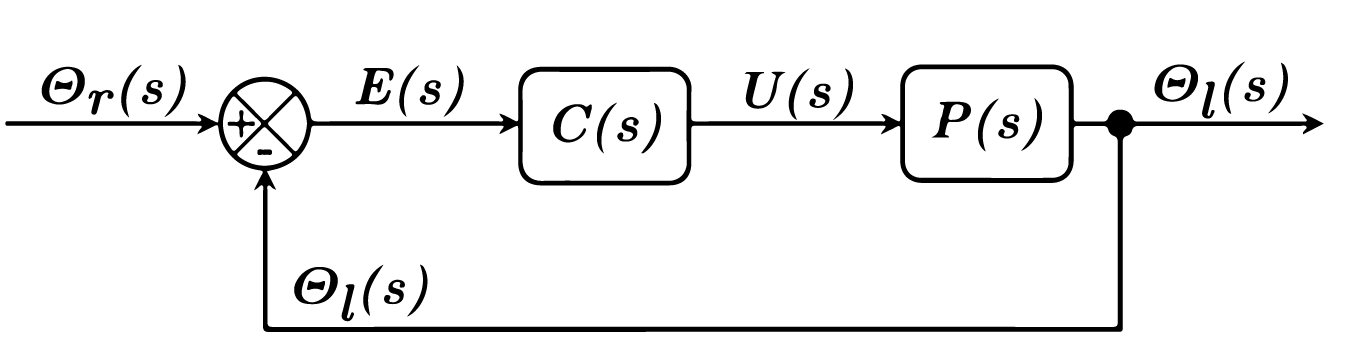
\includegraphics[width=0.6\textwidth]{servomotor_closed_loop_diagram}
    \caption{Diagram illustrating the key parameters in the dynamical model of the servomotor}
\end{figure}
The closed-loop system is shown in Figure 3.7, where the controller $C(s)$ is assumed to use a proportional control with gain $K_P$. The input of the closed-loop control is the commanded angle $\Theta_r(s)$, and the feedback signal is the load output shaft angle $\Theta_l(s)$. The error signal $E(s)$ is defined as the difference between the commanded angle and the actual output angle. The open-loop transfer function $P(s)$, is used to obtain the closed-loop transfer function $G(s)$, which relates the output angle $\Theta_l(s)$ to the commanded angle $\Theta_r(s)$:

\begin{equation} 
G(s) = \frac{\Theta_l(s)}{\Theta_r(s)} = \frac{\eta K_t K_P}{(RJ_{eq}s^2 + (Rb_{eq} + \eta N^2 K_t^2 K_P)s + \eta N K_t K_P)} 
\end{equation}

This transfer function characterizes the closed-loop behavior of the servo motor, taking into account the effects of the proportional control and the feedback loop.
Due to the limited time in our thesis we will use the parameters and transfer function identified in\cite{santanacob} which it uses a very unique method to determine the input and output angles of the servo therefore to be able to use the Matlab system identification toolbox:

\begin{equation} \frac{\Theta_l(s)}{\Theta_r(s)} = \frac{224.8}{s^2 + 22.33s + 225.4} 
\end{equation}
can also be represented in state space formula as:
\begin{equation}
\begin{bmatrix}
\Dot{\Theta_l}\\
\Ddot{\Theta_l}\\
\end{bmatrix}
=
\begin{bmatrix}
1\Dot{\Theta_l}\\
225.4\Theta_l + 22.33\dot{\Theta_l}\\
\end{bmatrix}
+ 
\begin{bmatrix}
0  \\
224.8 \\
\end{bmatrix}
\begin{bmatrix}
\Theta_r  \\
\end{bmatrix}
\end{equation}

\subsection{Linking Plate Inclination and Servo Motion}
There are several different ways to connect the motor to the plate that to convert the rotational move of the servomotor into a simple plate inclination, we have adopted the simplest method, such as the one shown in figure. 3.8, by the requirement of minimum inclination angle and due to the lack of availability of all parts in the market, we were able to obtain and construct the dimension shown in Table. 2 \\
\begin{figure}[h]
    \centering
    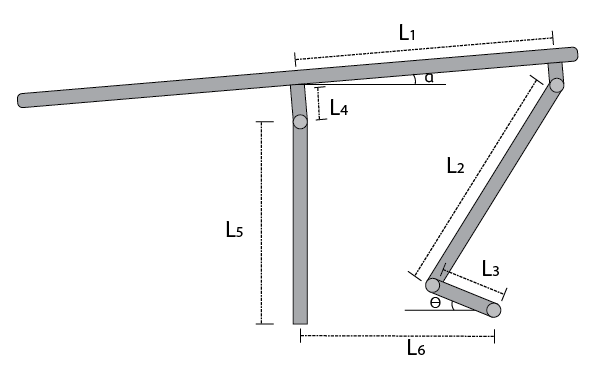
\includegraphics[width=0.8\textwidth]{actutation_platform_geometry.png}
    \caption{geometric illustration of the linkage between actuator and the plate of BPS}
\end{figure}

\begin{table}[h]
  \centering
  \caption{System dimensions in centimeter}
  \begin{tabular}{|c|c c c c c c|}
    \hline
    \hline
     X & L1 & L2 & L3 & L4 & L5 & L6 \\
    \hline
    Value & 9.5 & 24 & 1.5 & 5 & 22 & 13.4 \\
    \hline
    \hline
     Y & L1 & L2 & L3 & L4 & L5 & L6 \\
    \hline
    Value & 10 & 24 & 1.5 & 5 & 22 & 13 \\
    \hline
  \end{tabular}
\end{table}
The relation between the angle of rotation of the plate around the x axis \(\alpha\) and the angle of rotation of servomotor arm L3 \(\Theta\) is:
\begin{equation}
\sin{\Theta} = \frac{L_3}{L_1}\sin{\alpha}
\end{equation}
which can be represented as a constant gain \(K_l= \frac{L_3}{L_1}\), from Table. 2
\begin{equation}
K_{lx} = 0.158 \\\
K_{ly} = 0.150
\end{equation}
but the behaviour of the angles appears a Little different so we decided to map the inclination angle with the servo motor angle and determinee by the linear relationship regression the appropriate gain
the full table and details of mapping method found in Appendix C, and the new gain values we get is:
\begin{equation}
K_{lx} = 0.0445 \\\
K_{ly} = 0.0377
\end{equation}
The overall system equation taking in account the plant equation Eq. (3.39) (3.40) with the linkage gain Eq. (3.47) and the identified servomotor equation Eq. (3.43) can be represented as follows:
\begin{equation}
\frac{x}{\Theta_r}=\frac{70.1}{s^4+22.33s^3+225.4s^2}
\end{equation}
Which after state space transformation:
\begin{equation}
\begin{bmatrix}
\Dot{x_1}\\
\Ddot{x_2}\\
\Dot{x_3}\\
\Ddot{x_4}\\
\end{bmatrix}
=
\begin{bmatrix}
x_1\\
\frac{-5}{7}gx_3\\
x_4\\
-225.4x_x -22.33x_4\\
\end{bmatrix}
+ 
\begin{bmatrix}
0  \\
0 \\
0 \\
70.1
\end{bmatrix}
\begin{bmatrix}
\Theta_r  \\
\end{bmatrix}
\end{equation}
The system in Eq. (3.47)(3.48) is a fourth order transfer function, unstable due to the two poles in the origins as shown fig. 3.9, however it can be considered as a second order system since the other two poles in fig. 3.9 are in the left side far away from the origin so they have a little impact on the system behavior

\begin{figure}[h]
    \centering
    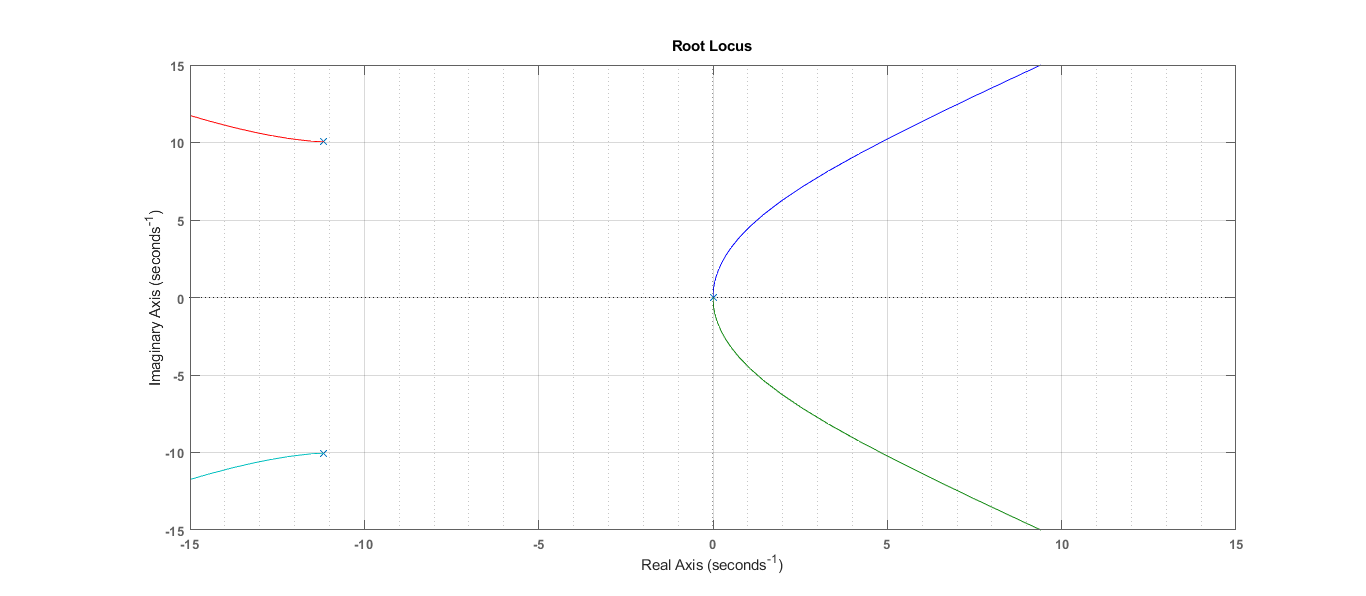
\includegraphics[width=1\textwidth]{RootLocus.png}
    \caption{Root Locus Analysis: Navigating Stability for BPS}
\end{figure}

